\documentclass{beamer}
\usepackage{polyglossia}
\usepackage{pgfpages}
\usepackage{mdframed}
\usepackage{tikz}
\usepackage{outlines}
\usepackage{setspace}
\usepackage{enumerate}
\usepackage{colonequals}
\usepackage{halloweenmath}
\usepackage{fontawesome5}
\usetheme{metropolis}


\newcommand{\NT}[1]{#1}
\newcommand{\T}[1]{#1}
\newcommand{\Term}[1]{\texttt{#1}}
\newcommand{\Arrow}{::=}
\newcommand{\Alphabet}{\Sigma}
\newcommand{\ItemDot}{\,\text{\textbullet}\,}
\newcommand{\ItemSep}{\enspace\:}
\newcommand{\Seq}{\,}
\newcommand{\Spc}{\,}
\newcommand{\Union}{\ |\ }
\newcommand{\Inter}{\ \&\ }
\newcommand{\Comp}{\lnot\,}
\newcommand{\Diff}{\mathrel{-}}
\newcommand{\Subclass}{U}
\newcommand{\Language}{\mathcal{L}}
\newcommand{\Spec}{\Xi}
\newcommand{\Kleene}[1]{{#1^*}}
\newcommand{\KleenePlus}[1]{#1^+}
\newcommand{\LblSep}{.\ }
\newcommand{\StartSymbol}{\NT{S}}
\newcommand{\EOF}{\Term{\$}}
\newcommand{\Middle}[2]{{#1_{#2}}}
\newcommand{\Call}{{\mathcal{C}}}

\newcommand{\Year}[1]{{$^{\text{\textquotesingle}#1}$}}
\newcommand{\YearD}[2]{{$^{\text{\textquotesingle}#1, \text{\textquotesingle}#2}$}}

\usetikzlibrary{automata, positioning, arrows, fit, matrix, shapes.geometric, shapes.misc, calc, decorations.text}

\setmainlanguage{slovenian}
\setotherlanguages{english}

%\setbeameroption{show only notes}
\setbeameroption{show notes on second screen=right}
\setbeamertemplate{note page}{
  %\insertvrule{\paperheight}{white}%
  \insertvrule{\paperheight}{note page.bg}%
  \vskip-0.95\paperheight%
  \usebeamercolor[fg]{note page}%
  (\insertframenumber) \insertframetitle%
  \insertnote%
}

\usepackage[binary-units]{siunitx}

\usepackage{tikz}
\usetikzlibrary{arrows.meta,decorations.pathmorphing,automata,positioning,arrows,fit,matrix,shapes.geometric,shapes.misc,shapes.symbols,calc,external,patterns}

\tikzset{
  every picture/.style={line width=0.8pt},
  node distance=2.4cm,
  vert/.style={draw, circle},
  every state/.append style={font=\footnotesize, minimum size=0.75cm, inner sep=0cm},
  pstate/.style={draw, rounded rectangle, font=\footnotesize, minimum width=1cm, inner sep=0.3cm},
  %every edge/.append style={thick},
  every label/.append style={font=\footnotesize},
  every node/.style={font=\footnotesize}
}

\usepackage{pgfplots}
\usepgfplotslibrary{external}
\usepgfplotslibrary{colorbrewer}
\pgfplotsset{
  layers/multilayer/.define layer set={
    background,
    main,
    foreground
  }{},
  set layers=multilayer
}


%\usepackage{pgfpages}
%\pgfpagesuselayout{4 on 1}[a4paper, landscape, border shrink=5mm]

\title{\large Generalizacija kontekstno zavednega pregledovanja za vse črkovne kontekstno neodvisne jezike}
\date{\today}
\author{Žiga Leber}
\institute{Laboratorij za programirne metodologije}
\titlegraphic{\includegraphics[height=1.2cm]{images/logo.pdf}}

\definecolor{university}{HTML}{00698F}
\definecolor{universitydark}{HTML}{003143}

\setbeamercolor{normal text}{%
  fg=universitydark,
  bg=black!2
}

\setbeamercolor{alerted text}{%
  fg=university
}

\selectlanguage{slovenian}

\begin{document}
\maketitle

\begin{frame}{Context}
  \centering
  \begin{tikzpicture}[tips=proper]
    \tikzset{
      ->,
      node distance=0.7cm,
      node/.style={},
      desc/.append style={font=\scriptsize},
    }
    \node (ptr) {PTR};
    \node[above=of ptr] (ast) {AST};

    \node[below=of ptr] (sppf) {SPPF};
    \node[below=of sppf] (text) {Text};

    \draw (ast.south east) edge[<-, bend left=50] node[right, desc] {Pruning} (ptr.north east);
    \draw (ast.south west) edge[->, bend right=50] node[left, desc] {Formatting} (ptr.north west);

    \draw (sppf.north) edge[->] node[right, desc] {Disambiguation} (ptr.south);

    \draw (text.north) edge[->, very thick] node[right, desc] {\textbf{Parsing}}  (sppf.south);
    \draw (text.north west) edge[<-, bend left=50] node[left, desc] {Concatenation} (ptr.south west);

    \draw (ast) edge[<-, loop above] node[above left, desc] {Structural editing} (ast);
    \draw (text) edge[<-, loop below] node[below right, desc] {Text editing} (text);
  \end{tikzpicture}

  \note[item]{The subject of this doctoral dissertation is a parsing architecture.}
  \note[item]{The architecture was developed for use in multiple representation editors.}
  \note[item]{Multiple representation editors are composed from multiple editing panes.}
  \note[item]{These can be structural or textual.}
  \note[item]{In structural editing we directly edit the abstract syntax tree, in textual text.}
\end{frame}

\begin{frame}
\includegraphics[height=0.9\textheight]{images/screenshot2.png}
  \note[item]{The practical applications are editors, with a block-based and a textual editor}
  \note[item]{An example of such editor is Poliglot.}
  \note[item]{Editing of the textual notation changes the textual and vice-versa.}
  \note[item]{It turns out that if you teach children just in block based editor they later cannot program in a textual programming language.}
\end{frame}

\begin{frame}{Idea}
  \begin{LARGE}
    {Combination of a scanner-based and a scannerless approach}\par
  \end{LARGE}
  \note[item]{Unified algorithm like in a scannerless approach, one automaton, one set of tables, one data structure for parsing, but still conceptually using a scanner.}
  \note[item]{The idea is to deconstruct scanner based parsing into its constituent parts, and reassemble them into a generalized algorithm.}
  \note[item]{Combination of LR and LR' interpretations, and limited form of non-canonical parsing.}
  \note[item]{The construction is the simplest possible that gives rise to such a parser.}
\end{frame}

\begin{frame}{Construction}
  \begin{enumerate}
    \item Regular right part grammar
    \item Construct the RTN (non-deterministic LR automaton, Brzozowski derivatives)
    \item Optimize
      \begin{itemize}
        \item \textsc{lr} for the parser section
        \item \textsc{earley1} for the scanner section
      \end{itemize}
    \item Enhance (cross-product construction)
    \item Extract enhanced productions
    \item Compute lookahead (\textsc{nullable}, \textsc{first}, \textsc{follow})
    \item Add non-canonical transitions
  \end{enumerate}

  \note[item]{The construction starts with RRPG, these are grammars with regular expression in the right-hand side.}
  \note[item]{The construction is the same as non-deterministic LR construction in Parsing Techniques.}
  \note[item]{The difference is I use Brzozowski derivatives, instead of DeRemer derivatives, that way intersection, difference and complement are supported as well.}
  \note[item]{LR is essentially a subset construction, where call transitions are collapsed into a loop, kernel and non-kernel items are joined.}
  \note[item]{Limited form of early construction, the kernel items and non-kernel items are separated by a transition.}
  \note[item]{Enhance, compute the cross product construction between unoptimized and optimized automaton.}
  \note[item]{Compute the lookahead from NULLABLE, FIRST, FOLLOW and add non-canonical transitions.}
\end{frame}

\begin{frame}{Regular right part grammar}
  \begin{equation*}
    \begin{aligned}
      \_\LblSep\NT{S} &\Arrow_0 \NT{A} \Union \T{b} \Spc \Kleene{(\T{c} \Spc \T{b})}\\
      \_\LblSep\NT{A} &\Arrow_1 \T{b} \Spc \T{c}
    \end{aligned}
    \hspace{3em}
    \begin{aligned}
      \_\LblSep\T{b} &\Arrow_2 \Term{x}\\
      \_\LblSep\T{c} &\Arrow_3 \Term{y}
    \end{aligned}
  \end{equation*}

  \note[item]{The right hand sides are regular expressions.}
  \note[item]{The productions are labeled, the labels later end up labeling the sets of children in the parse forest.}
  \note[item]{In this case all productions are labeled with the null label, which means that nodes that end up labeled with this label get pruned.}
  \note[item]{And they are indexed, numbered sequentially.}

\end{frame}

\begin{frame}{Unoptimized RTN}
  \resizebox{!}{0.8\textheight}{
  \begin{tikzpicture}[tips=proper, node distance=2cm and 2cm, initial text=]
    \node [state, initial] (0) {0};
    \node [state, right of=0] (1) {1};
    \node [state, accepting, right of=1] (2) {2};

    \node [state, below of=1] (3) {3};

    \node [state, right of=3] (10) {10};

    \node [state, below of=10] (11) {11};

    \node [state, below of=3] (4) {4};

    \node [state, below of=4] (5) {5};

    \node [state, below of=5] (6) {6};

    \node [state, below of=6] (7) {7};

    \node [state, right of=6] (8) {8};
    \node [state, below of=8] (9) {9};

    \node [state, right of=11] (12) {12};
    \node [state, right of=12] (13) {13};

    \node [left=0.5 of 5, label={$\_\LblSep \NT{S}$}] (n1) {};

    \node [right=0.5 of 10, label={$\_\LblSep \NT{S}$}] (n2) {};
    \node [right=0.5 of 13, label={$\_\LblSep \NT{A}$}] (n3) {};
    \node [right=0.5 of 7, label={$\_\LblSep \T{b}$}] (n4) {};
    \node [right=0.5 of 9, label={$\_\LblSep \T{c}$}] (n5) {};

    \draw(0) edge[->] node[above]{$\StartSymbol$} (1);
    \draw(1) edge[->] node[above]{$\EOF$} (2);
    \draw(2) edge[->, loop above] node[above]{$\EOF$} (2);

    \draw(0) edge[->] node[auto]{$\Middle{\Call}{\NT{S}}$} (3);

    \draw(3) edge[->] node[auto]{$\Middle{\Call}{\NT{A}}$} (11);

    \draw(3) edge[->] node[auto]{$\NT{A}$} (10);

    \draw(11) edge[->] node[auto]{$\T{b}$} (12);
    \draw(12) edge[->] node[auto]{$\T{c}$} (13);

    \draw(3) edge[->] node[auto]{$\T{b}$} (4);

    \draw(4) edge[->, bend left] node[auto]{$\T{c}$} (5);
    \draw(5) edge[->, bend left] node[auto]{$\T{b}$} (4);

    \draw(5) edge[->] node[auto]{$\Middle{\Call}{\T{b}}$} (6);

    \draw(6) edge[->] node[auto]{$\Term{x}$} (7);
    \draw(8) edge[->] node[auto]{$\Term{y}$} (9);

    \draw(3) edge[->, bend right=50] node[left]{$\Middle{\Call}{\T{b}}$} (6);

    \draw(11) edge[->, bend left] node[left]{$\Middle{\Call}{\T{b}}$} (6);
    \draw(4) edge[->, bend left] node[left]{$\Middle{\Call}{\T{c}}$} (8);

    \draw(12) edge[->, bend left] node[left]{$\Middle{\Call}{\T{c}}$} (8);

    \draw(5) edge[->] (n1);
    \draw(10) edge[->] (n2);
    \draw(13) edge[->] (n3);
    \draw(7) edge[->] (n4);
    \draw(9) edge[->] (n5);
  \end{tikzpicture}
  }
  \note[item]{Each state corresponds to an item in a LR automaton.}
  \note[item]{As a transition is made a derivative is computed.}
  \note[item]{If DeRemer derivatives were used that would mean that the dot is moved over the symbol.}
  \note[item]{With Brzozowski derivatives, a regular expression is computed with the symbol removed from the beginning.}
  \note[item]{Call transitions are added when there are non-terminals at the beginning of the regular expression.}
\end{frame}

\begin{frame}{Optimized RTN}
  \resizebox{!}{0.8\textheight}{
  \begin{tikzpicture}[tips=proper, node distance=2cm and 2cm, initial text=]
    \node [state, initial] (0) {0};
    \node [state, right of=0] (1) {1};
    \node [state, accepting, right of=1] (2) {2};

    \node [state, below of=1] (3) {3};
    \node [state, below of=3] (4) {4};
    \node [state, below of=4] (5) {5};
    \node [state, below of=5] (6) {6};
    \node [state, below of=6] (7) {7};

    \node [state, left of=5] (8) {8};
    \node [state, left of=8] (9) {9};

    \node [state, right of=6] (10) {10};
    \node [state, below of=10] (11) {11};

    \node [right=0.5 of 5, label={below:$\_\LblSep \NT{A}$}] (n1) {};
    \node [right=0.5 of 4, label={$\_\LblSep \NT{S}$}] (n2) {};
    \node [left=0.5 of 6, label={$\_\LblSep \NT{S}$}] (n3) {};
    \node [right=0.5 of 11, label={$\_\LblSep \T{c}$}] (n4) {};
    \node [left=0.5 of 9, label={$\_\LblSep \T{b}$}] (n5) {};
    \node [right=0.5 of 3, label={$\_\LblSep \NT{S}$}] (n6) {};

    \draw(0) edge[->] node[above]{$\StartSymbol$} (1);
    \draw(1) edge[->] node[above]{$\EOF$} (2);
    \draw(2) edge[->, loop above] node[above]{$\EOF$} (2);

    \draw(0) edge[->, bend right=10] node[auto]{$\NT{A}$} (3);

    \draw(0) edge[->, bend right=10] node[auto]{$\T{b}$} (4);

    \draw(4) edge[->, bend left=10] node[auto]{$\Middle{\Call}{\T{c}}$} (10);

    \draw(6) edge[->] node[auto]{$\Middle{\Call}{\T{c}}$} (10);

    \draw(7) edge[->, bend left=25] node[auto]{$\Middle{\Call}{\T{b}}$} (8);
    \draw(5) edge[->] node[auto]{$\Middle{\Call}{\T{b}}$} (8);
    \draw(0) edge[->] node[auto]{$\Middle{\Call}{\T{b}}$} (8);

    \draw(4) edge[->] node[auto]{$\T{c}$} (5);
    \draw(5) edge[->] node[auto]{$\T{b}$} (6);

    \draw(7) edge[->, bend right] node[right]{$\T{b}$} (6);
    \draw(6) edge[->, bend right] node[left]{$\T{c}$} (7);

    \draw(10) edge[->] node[auto]{$\Term{y}$} (11);
    \draw(8) edge[->] node[auto]{$\Term{x}$} (9);

    \draw (0) edge[->, loop above] node[auto] {$\Middle{\Call}{\NT{S}\ \NT{A}}$} (0);

    \draw(5) edge[->] (n1);
    \draw(4) edge[->] (n2);
    \draw(6) edge[->] (n3);
    \draw(11) edge[->] (n4);
    \draw(9) edge[->] (n5);
    \draw(3) edge[->] (n6);
  \end{tikzpicture}
  }
  \note[item]{The parser section are sub-RTNs reachable using call transitions with syntactic non-terminals, the scanner section are sub-RTNs reachable using call transitions with lexical non-terminals.}
  \note[item]{The call transitions for syntactic non-terminals are collapsed into a loop.}
  \note[item]{The call transitions for lexical non-terminals are collapsed into a single transition.}
  \note[item]{Scanner section is the same as constructing an automaton for context-aware scanning for each LR state and connecting it with a call transition.}
\end{frame}

\begin{frame}{Enhanced RTN}
  \resizebox{!}{0.8\textheight}{
  \begin{tikzpicture}[tips=proper, node distance=1.4cm and 1.5cm, initial text=]
    \node [pstate] (0) {$0\quad 0$};
    \node [pstate, right=of 0] (1) {$1\quad 1$};
    \node [pstate, right=of 1] (2) {$2\quad 2$};
    \node [pstate, below=of 0] (3) {$0\quad 3$};
    \node [pstate, right=of 3] (4) {$4\quad 4$};
    \node [pstate, right=of 4] (5) {$5\quad 5$};
    \node [pstate, right=of 5] (6) {$6\quad 4$};
    \node [pstate, right=of 6] (7) {$7\quad 5$};

    \node [pstate, below=of 3] (8) {$0\quad 11$};
    \node [pstate, below=of 8] (9) {$4\quad 12$};
    \node [pstate, below=of 9] (10) {$5\quad 13$};
    \node [pstate, left=of 3] (11) {$3\quad 10$};
    \node [pstate, below=of 4] (12) {$8\quad 6$};
    \node [pstate, below=of 12] (13) {$9\quad 7$};

    \node [pstate, right=of 13] (14) {$10\quad 8$};
    \node [pstate, below=of 14] (15) {$11\quad 9$};

    \draw(0) edge[->] node[auto]{$(0, \NT{S})$} (1);
    \draw(1) edge[->] node[auto]{$(1, \Term{\$})$} (2);
    \draw(2) edge[->, loop above] node[auto]{$(2, \Term{\$})$} (2);

    \draw(0) edge[->] node[auto]{$(0, \Middle{\Call}{\NT{S}})$} (3);
    \draw(3) edge[->] node[auto]{$(0, \T{b})$} (4);
    \draw(4) edge[->] node[auto]{$(4, \T{c})$} (5);
    \draw(5) edge[->] node[auto]{$(5, \T{b})$} (6);
    \draw(6) edge[->, bend left] node[auto]{$(6, \T{c})$} (7);
    \draw(7) edge[->, bend left] node[auto]{$(7, \T{b})$} (6);

    \draw(3) edge[->] node[auto]{$(0, \Middle{\Call}{\NT{A}})$} (8);
    \draw(8) edge[->] node[auto]{$(0, \T{b})$} (9);
    \draw(9) edge[->] node[auto]{$(4, \T{c})$} (10);

    \draw(3) edge[->] node[auto]{$(0, \NT{A})$} (11);
    \draw(12) edge[->] node[auto]{$(8, \Term{x})$} (13);


    \draw(14) edge[->] node[auto]{$(10, \Term{y})$} (15);

    \draw(3) edge[->] node[auto]{$(0, \Middle{\Call}{\T{b}})$} (12);
    \draw(8) edge[->] node[auto]{$(0, \Middle{\Call}{\T{b}})$} (12);
    \draw(5) edge[->] node[auto]{$(5, \Middle{\Call}{\T{b}})$} (12);
    \draw(7) edge[->, controls=+(-90:2) and +(0:3)] node[auto]{$(7, \Middle{\Call}{\T{b}})$} (12);

    \draw(9) edge[->, bend right] node[below]{$(4, \Middle{\Call}{\T{c}})$} (14);
    \draw(6) edge[->] node[auto]{$(6, \Middle{\Call}{\T{c}})$} (14);
    \draw(4) edge[->] node[auto]{$(4, \Middle{\Call}{\T{c}})$} (14);
  \end{tikzpicture}
  }
  \note[item]{We compute the cross-product construction, possible because the call transitions are collapsed into a loop.}
  \note[item]{The enhanced automaton can be used to compute the entire right context.}
\end{frame}

\begin{frame}{Extracted enhanced productions}
  \resizebox{!}{0.7\textheight}{
  \begin{tikzpicture}[tips=proper, node distance=1.4cm and 1.5cm, initial text=]
    \begin{scope}
      \node [pstate, label={above left:(0, \NT{S})}] (0) {$0\quad 3$};
      \node [pstate, right=of 0] (1) {$4\quad 4$};
      \node [pstate, below right=of 0] (2) {$3\quad 10$};
      \node [pstate, right=of 1] (3) {$5\quad 5$};
      \node [pstate, right=of 3] (4) {$6\quad 4$};
      \node [pstate, right=of 4] (5) {$7\quad 5$};

      \draw(0) edge[->] node[auto]{$(0, \T{b})$} (1);
      \draw(0) edge[->] node[auto]{$(0, \NT{A})$} (2);
      \draw(1) edge[->] node[auto]{$(4, \T{c})$} (3);
      \draw(3) edge[->] node[auto]{$(5, \T{b})$} (4);
      \draw(4) edge[->, bend left] node[auto]{$(6, \T{c})$} (5);
      \draw(5) edge[->, bend left] node[auto]{$(7, \T{b})$} (4);
    \end{scope}
    \begin{scope}[shift={(0, -4)}]
      \node [pstate, label={above left:(0, \NT{A})}] (0) {$0\quad 11$};
      \node [pstate, right=of 0] (1) {$4\quad 12$};
      \node [pstate, right=of 1] (2) {$5\quad 13$};

      \draw(0) edge[->] node[auto]{$(0, \T{b})$} (1);
      \draw(1) edge[->] node[auto]{$(4, \T{c})$} (2);
    \end{scope}
    \begin{scope}[shift={(0, -6)}]
      \node [pstate, label={above left:(0, \T{b})\ (5, \T{b})\ (7, \T{b})}] (0) {$8\quad 6$};
      \node [pstate, right=of 0] (1) {$9\quad 7$};

      \draw(0) edge[->] node[auto]{$(8, \Term{x})$} (1);
    \end{scope}
    \begin{scope}[shift={(0, -8)}]
      \node [pstate, label={above left:(4, \T{c})\ (6, \T{c})}] (0) {$10\quad 8$};
      \node [pstate, right=of 0] (1) {$11\quad 9$};

      \draw(0) edge[->] node[auto]{$(10, \Term{y})$} (1);
    \end{scope}
  \end{tikzpicture}
  }
  \note[item]{Enhanced productions are extracted from the enhanced RTN.}
  \note[item]{Then NULLABLE, FIRST, FOLLOW are computed, which are used compute the lookahead.}
  \note[item]{The reduce lookahead is computed, by first computing lookback and then FOLLOW of the enhanced symbol.}
  \note[item]{In state 6, for item 4 the lookahead is computed as FOLLOW(0, A).}
\end{frame}

\begin{frame}{Non-canonical RTN}
  \resizebox{!}{0.8\textheight}{
  \begin{tikzpicture}[tips=proper, node distance=2cm and 2cm, initial text=]
    \node [state, initial] (0) {0};
    \node [state, right of=0] (1) {1};
    \node [state, accepting, right of=1] (2) {2};

    \node [state, below of=1] (3) {3};
    \node [state, below of=3] (4) {4};
    \node [state, below of=4] (5) {5};
    \node [state, below of=5] (6) {6};
    \node [state, below of=6] (7) {7};

    \node [state, left of=5] (8) {8};
    \node [state, left of=8] (9) {9};

    \node [state, right of=6] (10) {10};
    \node [state, below of=10] (11) {11};

    \node [right=0.5 of 5, label={below:$\_\LblSep \NT{A}$}] (n1) {};
    \node [right=0.5 of 4, label={$\_\LblSep \NT{S}$}] (n2) {};
    \node [left=0.5 of 6, label={$\_\LblSep \NT{S}$}] (n3) {};
    \node [right=0.5 of 11, label={$\_\LblSep \T{c}$}] (n4) {};
    \node [left=0.5 of 9, label={$\_\LblSep \T{b}$}] (n5) {};
    \node [right=0.5 of 3, label={$\_\LblSep \NT{S}$}] (n6) {};

    \draw(0) edge[->] node[above]{$\StartSymbol$} (1);
    \draw(1) edge[->] node[above]{$\EOF$} (2);
    \draw(2) edge[->, loop above] node[above]{$\EOF$} (2);

    \draw(0) edge[->, bend right=10] node[auto]{$\NT{A}$} (3);

    \draw(0) edge[->, bend right=10] node[auto]{$\T{b}$} (4);

    \draw(4) edge[->, bend left=10] node[auto]{$\Middle{\Call}{\T{c}}$} (10);

    \draw(6) edge[->] node[auto]{$\Middle{\Call}{\T{c}}$} (10);

    \draw(7) edge[->, bend left=25] node[auto]{$\Middle{\Call}{\T{b}}$} (8);
    \draw(5) edge[->] node[auto]{$\Middle{\Call}{\T{b}}$} (8);
    \draw(0) edge[->] node[auto]{$\Middle{\Call}{\T{b}}$} (8);

    \draw(4) edge[->] node[auto]{$\T{c}$} (5);
    \draw(5) edge[->] node[auto]{$\T{b}$} (6);

    \draw(7) edge[->, bend right] node[right]{$\T{b}$} (6);
    \draw(6) edge[->, bend right] node[left]{$\T{c}$} (7);

    \draw(10) edge[->] node[auto]{$\Term{y}$} (11);
    \draw(8) edge[->] node[auto]{$\Term{x}$} (9);

    \draw (0) edge[->, loop above] node[auto] {$\Middle{\Call}{\NT{S}\ \NT{A}}$} (0);

    \draw(5) edge[->] (n1);
    \draw(4) edge[->] (n2);
    \draw(6) edge[->] (n3);
    \draw(11) edge[->] (n4);
    \draw(9) edge[->] (n5);
    \draw(3) edge[->] (n6);
  \end{tikzpicture}
  }
  \note[item]{In this case there is no difference between the optimized RTN and the non-canonical one.}
  \note[item]{In general in each reduce state, add a call transition for each lookahead (state, symbol).}
  \note[item]{That way there is a call transition for each lookahead symbol as well.}
  \note[item]{This is a special case of non-canonical parsing.}
\end{frame}

\begin{frame}[t]{GLR}
  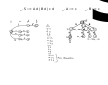
\includegraphics{images/glr1.pdf}
  \note[item]{There is a shift/reduce and a reduce/reduce conflict in state 1.}
  \note[item]{The algorithm tries all possibilities.}
  \note[item]{The reduce is performed by scanning back the stack for 1 step.}
  \note[item]{The GSS contains all possible stacks, except that common prefixes and suffixes are combined.}
  \note[item]{All stacks start with a 0, and in the graph the 0 are combined in one vertex.}
\end{frame}

\begin{frame}[t]{RNGLR}
  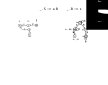
\includegraphics{images/rnglr1.pdf}
  \note[item]{The right nulled production pose a problem for the parser.}
  \note[item]{The reductions involving the right nulled production are performed using short-circuited reduce actions.}
  \note[item]{In state 1 the reduce action can be performed by scanning back the stack for 1 step.}
  \note[item]{The null reduce action is performed after the fact.}
\end{frame}

\begin{frame}[t]{RNGLR}
  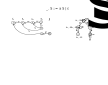
\includegraphics{images/rnglr2.pdf}
  \note[item]{To see why it was necessary to add short-circuited reduce actions, lets see how the algorithm keeps track of which reduce moves still need to be performed.}
  \note[item]{The reduce moves are only performed for newly added edges to a vertex.}
\end{frame}

\begin{frame}[t]{RNGLR}
  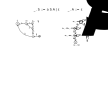
\includegraphics{images/rnglr3.pdf}
  \note[item]{Here the reduce move would also need to be performed for an edge added to an ancestor from state 3.}
  \note[item]{That is one solution, however it is less efficient.}
  \note[item]{Short-circuiting the reduce actions allows the reduce actions to still only be performed for newly added edges to a vertex.}
\end{frame}

\begin{frame}[t]{RNGSGLR}
  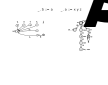
\includegraphics{images/rngsglr1.pdf}
  \note[item]{The interpretation changes in the scanner section. The parser section works like RNGLR.}
  \note[item]{Instead of going like () <- () <- (), it goes like () <- (), <-(), <- ().}
  \note[item]{If there is an edge "a" in the RTN, an order link is added, they indicate that a shift action is possible from a state.}
  \note[item]{"a" is shifted, then a reduction is performed in state 3, scan back the stack for 1 step.}
\end{frame}

\begin{frame}[t]{RNGSGLR}
  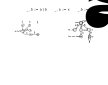
\includegraphics{images/rngsglr2.pdf}
  \note[item]{There is match/match conflict in state 9.}
  \note[item]{The problem can be solved using a Schrodingers token.}
  \note[item]{Shift action action is performed for both matches. This techinque has already been mentioned by Tomita in the original GLR book.}
  \note[item]{The edges in the RTN can be labeled with multiple symbols.}
  \note[item]{As a result there are multiple symbols on the GSS edges.}
\end{frame}

\begin{frame}[t]{RNGSGLR}
  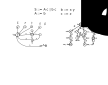
\includegraphics{images/rngsglr3.pdf}
  \note[item]{The items are labeled with a distance from the start, that way only the states with the same distance get merged.}
  \note[item]{If the regular expression describes a lanuge of infinite size infinity is used as the distance, that way a loop is created in the RTN.}
  \note[item]{In state 4 there are two different reduction paths.}
  \note[item]{The shift action is performed from states 7 and 3.}
\end{frame}

\begin{frame}[t]{RNGSGLR}
  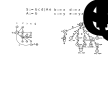
\includegraphics{images/rngsglr4.pdf}
  \note[item]{There is a match/read conflict in state 18.}
  \note[item]{The problem is solved using fractional lookahead.}
  \note[item]{The reduce actions are performed using predictions as lookahead.}
  \note[item]{The reduce action can only be performed with "e" as lookahead.}
  \note[item]{That way the reduce actions are performed to completition after the first match is found.}
\end{frame}

\begin{frame}[t]{RNGSGLR}
  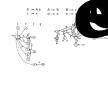
\includegraphics{images/rngsglr5.pdf}
  \note[item]{The order link is propagated from state 3, to state 7, to state 8.}
  \note[item]{Then the order link is propagated from state 7 to state 9.}
\end{frame}

\begin{frame}[t]{RNGSGLR}
  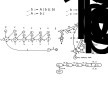
\includegraphics{images/rngsglr6.pdf}
  \note[item]{The reduction is performed by scanning back the stack using an automaton.}
  \note[item]{The automaton is constructed from an enhanced production by reversing the transitions.}
  \note[item]{The states and symbols from the transitions are matched with the states on vertices and symbols on edges in the GSS.}
\end{frame}

\begin{frame}[t]{RNGSGLR}
  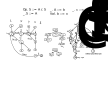
\includegraphics{images/rngsglr7.pdf}
  \note[item]{The labels end up labeling the sets of children in the parse forest.}
  \note[item]{After disambiguation, the nodes with the null label are pruned, giving the abstract syntax tree.}
  \note[item]{In this example no disambiguation was needed.}
\end{frame}

\begin{frame}
  \begin{huge}
  Thank you for your attention!\\[0.8em]
  \end{huge}
  \begin{Large}
  \faGithub\ brokenpylons/te
  \end{Large}
\end{frame}


\end{document}

